% Template para Proposta e TCC da EST/UEA -
% Padrão para os cursos do Núcleo de Computação
%
% Elaborado por Elloá B. Guedes
% Adaptado da versão elaborada por:
%                   Jucimar Maia Jr.
%
% Versão 1.3 - 15 de julho de 2022
%
\documentclass[a4paper,titlepage,12pt]{report}


\usepackage[utf8]{inputenc}
\usepackage[OT1]{fontenc}
\usepackage{ae}
\usepackage[brazil]{babel}
\usepackage{a4wide}
\usepackage{comment}
\usepackage[pdftex]{graphicx,color}
\usepackage{graphics}
\usepackage{cite}
\usepackage{longtable}
\usepackage{float}
\usepackage{fancyvrb}
\usepackage{fancyhdr}
\usepackage{setspace}
\usepackage{amsmath}
\usepackage{lscape}
\usepackage{textcase}
\usepackage{anysize}
\usepackage{setspace}
\usepackage{booktabs}
\usepackage{url}
\usepackage{subfig}
\usepackage{cite}
\usepackage[alf]{abntex2cite}
\usepackage{pdfpages}

\marginsize{20mm}{20mm}{20mm}{15mm}


%% Cabeçalhos
\renewcommand{\topfraction}{1}
\renewcommand{\bottomfraction}{1}
\renewcommand{\floatpagefraction}{1}
\renewcommand{\textfraction}{0}
%\renewcommand{\baselinestretch}{2}
\doublespacing %espaçamento duplo
\sloppy

%% Nomes
\floatstyle{plain}  %%% tipos: plain, boxed, ruled
\newfloat{codigo}{tbp}{lop}[section]
\floatname{codigo}{Código}

%%% nome para ser usado no sumário

\newcommand{\listofcodename}{Lista de C\'{o}digos}



% RESUMO ----------------------------------------------------------------------------------------------------------------------------------------------------------------------

\newcommand{\resumo}[1]{
\begin{center} \LARGE \bf Resumo \end{center}

\vskip 4em
\input{#1}

\newpage

}

% ABSTRACT ----------------------------------------------------------------------------------------------------------------------------------------------------------------------

\newcommand{\abstractt}[1]{
\begin{center} \LARGE \bf Abstract \end{center}

\vskip 4em
\input{#1}

\newpage

}

% Sumário -----------
\newcommand{\sumario}{
\renewcommand{\contentsname}{Sum\'{a}rio}
\tableofcontents
\addcontentsline{toc}{chapter}{\listtablename}
\listoftables

\newpage
\addcontentsline{toc}{chapter}{\listfigurename}
\listoffigures
\addcontentsline{toc}{chapter}{\listofcodename}
\listof{codigo}{\listofcodename}  % Lista de Códigos

\clearpage
}

\pagestyle{plain}

\newcommand{\folhaRosto}[5]{

\thispagestyle{empty}
\begin{center}
\textbf{\\[0.4em]\MakeUppercase{#2} \\[5cm]}
\textbf{\MakeUppercase{#1}\\[96pt]}

\end{center}

\hspace*{8cm}
\begin{minipage}{8cm}
Trabalho de Conclus\~{a}o de Curso
apresentado \`{a} banca avaliadora do Curso de Engenharia de Computa\c{c}\~{a}o, da
Escola Superior de Tecnologia, da Universidade do Estado do Amazonas, como
pr\'e-requisito para obten\c{c}\~{a}o do t\'{\i}tulo de Engenheiro de Computa\c{c}\~{a}o.\\[40pt]
\end{minipage}

\begin{center}
Orientador(a): #3 \\[12ex]
Manaus -- #4 -- #5\\
\end{center}


\pagenumbering{roman}
\newpage
}




%% Preencha aqui os seguintes dados
\def \titulo{Título do seu Trabalho de Conclusão de Curso}
\def \orientador{Prof. Dr. Nome Completo do Orientador}
\def \nome{Nome completo não abreviado do aluno}
\def \mes{Julho}
\def \ano{2022}

\begin{document}

\folhaRosto{\titulo}{\nome}{\orientador}{\mes}{\ano}

% Edite os seguintes arquivos para alterar as informações necessárias
\begin{center} \LARGE \bf Ficha Catalográfica \end{center}


\begin{enumerate}
    \item Estas instruções \textbf{não} devem ser entregues aos avaliadores do trabalho nas ocasiões dos TCCs 1 e 2. Portanto, comente a linha que importa este arquivo;
    \item A ficha catalográfica deve ser elaborada após a defesa do TCC2, quando você concluir as correções sugeridas pela banca e validar a versão final com o/a professor(a) orientador(a);
    \item Acessar \url{http://repositorioinstitucional.uea.edu.br:8080/ficha/ficha_catalografica.php} e preencher as informações requeridas para elaborar a ficha catalográfica;
    \item Incluir o pdf gerado na subpasta \emph{source} com o nome \texttt{ficha.pdf};
    \item Apagar todo o conteúdo deste arquivo e deixar apenas o comando a seguir:
    \begin{verbatim}
        \includepdf[pages=-]{./source/ficha.pdf}
    \end{verbatim}
\end{enumerate}

\newpage

\begin{center} \LARGE \bf Folha de Aprovação \end{center}


\begin{enumerate}
    \item Estas instruções \textbf{não} devem ser entregues aos avaliadores do trabalho nas ocasiões dos TCCs 1 e 2. Portanto, comente a linha que importa este arquivo;
    \item Após a defesa do TCC2, efetue as correções indicadas pela banca;
    \item Valide a versão final do trabalho com seu/sua orientador(a). Ele/Ela irá entregar uma carta de anuência ao coordenador da disciplina de TCC2 indicando estar de acordo com a versão final produzida;
    \item O responsável pela disciplina de TCC2 irá lhe entregar digitalmente um documento PDF com as assinaturas e aprovação dos integrantes da banca;
    \item O referido arquivo deve ser adicionado na pasta source com o nome \texttt{assinaturas.pdf};
    \item Todo o conteúdo deste arquivo deve ser retirado e substituído pelo seguinte comando:

   \begin{verbatim}
       \includepdf[pages=-]{./source/assinaturas.pdf}
   \end{verbatim}
\end{enumerate}

\newpage



% Indique onde esta o arquivo do resumo
\resumo{./files/resumo.tex}
% Idem para o abstract
\abstractt{./files/abstract.tex}


\sumario

% Configuração de cabeçalhos
\pagestyle{fancy}
\renewcommand{\chaptermark}[1]{\markboth{#1}{}}
\renewcommand{\sectionmark}[1]{\markright{#1}}
\renewcommand{\headrulewidth}{0.5pt}
\newcommand{\rom}{\fontfamily{cmr}\fontseries{m}\fontsize{10}{12}\selectfont}
\fancyhf{} \fancyhead[LE,RO]{\rom\thepage}
\fancyhead[LO]{\rom\rightmark} \fancyhead[RE]{\rom\leftmark}
\fancypagestyle{plain}{
    \fancyhead{} % get rid of headers
    \renewcommand{\headrulewidth}{0pt} % and the line
 }


\pagenumbering{arabic}



% Seus capítulos vão aqui --------
\chapter{Exemplo}

\section{Tabela com o Pacote Booktabs}

Um exemplo de tabela com o pacote booktabs pode ser visto na Tabela \ref{tabela:exemplo}. A explicação das tabelas sempre vem em cima e esse padrão deve ser respeitado. A numeração é automática e a inserção no índice também. Legal né? \cite{Bennett:QuantumInformationSurvey}

Basta quebrar uma linha para criar um novo parágrafo. Neste parágrafo vou contar que tabelas no \LaTeX dão um pouco de trabalho, mas nada que com paciência não se resolva. Veja os links com dicas que coloquei nos comentários do arquivo \texttt{index.tex}.

\begin{table}[ht!]
\caption{Esta é uma tabela básica em \LaTeX com o pacote booktabs.} \label{tabela:exemplo}
\center{
\begin{tabular}{cccc}
\toprule
Parte 1 & Parte 2 & Parte 3 & Parte 4\\
\midrule
0,415 & 1,365 & 1,98 & 2,05\\
1,36  & 45,5  & 7,98 & 3,01\\
2,36  & 1,35  & 0,15 & 5,32\\
\bottomrule
\end{tabular}}
\end{table}



\section{Inserção de Figuras}

Você pode inserir figuras JPG no \LaTeX! Veja o caso da Figura \ref{fig:exemplo}. Se você quiser outras configurações e dicas, veja o seguinte endereço: \url{http://en.wikibooks.org/wiki/LaTeX/Floats,_Figures_and_Captions}.

A explicação da figura sempre vem embaixo da mesma. Isto aqui é um novo parágrafo apenas para ilustrar a idéia geral de como escrever.

\begin{figure}[H]
\centering
\caption{Um exemplo de figura JPG inserida no \LaTeX.} \label{fig:exemplo}
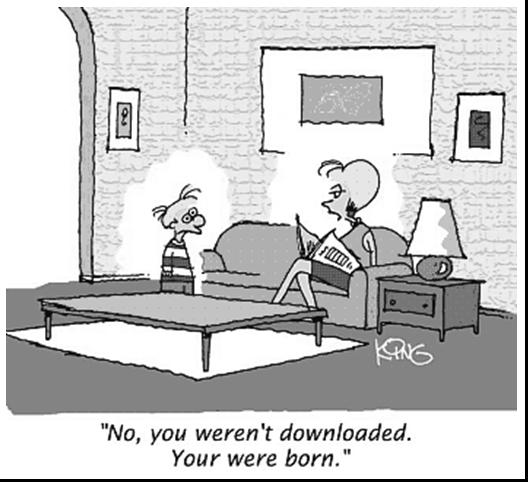
\includegraphics[width=0.4\textwidth]{./img/exemplo.jpg}\\
\small{Elaborado pelo autor.}
\end{figure}

Pode inserir várias figuras lado a lado também. Um exemplo está reproduzido a seguir.

\begin{figure}[H]
  \centering
  \caption{Canal clássico cuja obtenção da capacidade erro-zero é não-trivial.}
  \subfloat[\ ]{\label{fig:exG5}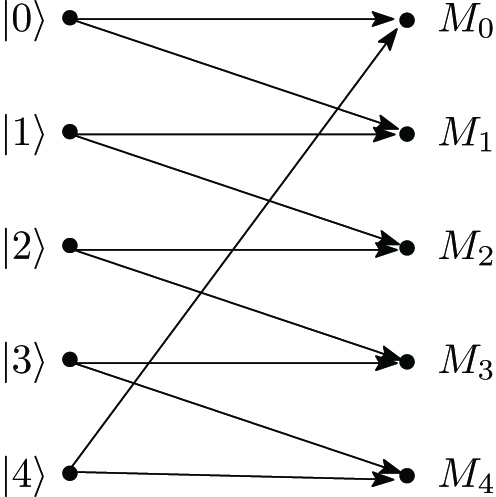
\includegraphics[width=0.3\textwidth]{./img/001}}
  \hspace{0.5cm}
  \subfloat[\ ]{\label{fig:exG52}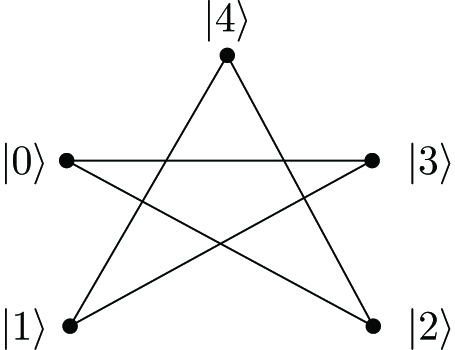
\includegraphics[width=0.3\textwidth]{./img/002}}
  \hspace{0.5cm}
  \subfloat[\ ]{\label{fig:exG53}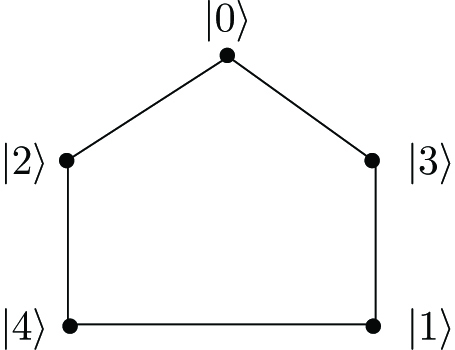
\includegraphics[width=0.3\textwidth]{./img/003}}\\
  \small{Elaborado por Bacon}
\end{figure}

\section{Referências Bibliográficas no Padrão ABNT}

Para gerar versões corretas do \textsc{Bib}\TeX das suas referências, recomenda-se usar o DOI no caso de artigos e o ISBN no caso de livros. Em posse dessas informações, consulte os seguintes links:

\begin{enumerate}
    \item \url{https://www.bibtex.com/c/doi-to-bibtex-converter/}
    \item \url{https://www.bibtex.com/c/isbn-to-bibtex-converter/}
    \item \url{http://doi-to-bibtex-converter.herokuapp.com/}
    \item \url{https://www.doi2bib.org/}
\end{enumerate}

Para saber mais sobre os tipos de referências \textsc{Bib}\TeX e seus significados, consultar a documentação oficial em \url{https://www.bibtex.com/e/entry-types/}.

Este template está integrado com o pacote \texttt{abnt2cite} que produz as referências no padrão ABNT NBR 6023.

\chapter{Título do Quarto Capítulo}


Vivamus ultricies tincidunt lacus ut pharetra. Sed fringilla hendrerit tempus. Suspendisse potenti. Cras hendrerit tortor ac est condimentum pellentesque. Morbi pretium lectus nec sapien laoreet eu malesuada diam adipiscing. Aliquam nisl ipsum, fermentum ut aliquam nec, varius sit amet nisi. Pellentesque interdum cursus malesuada. Vestibulum ante ipsum primis in faucibus orci luctus et ultrices posuere cubilia Curae; Nullam malesuada bibendum tortor, ut bibendum lorem varius eu. In eros orci, volutpat ut facilisis sit amet, commodo quis nulla.

Sed lectus metus, mollis nec vulputate id, imperdiet eget urna. Nam ut dolor at metus venenatis suscipit et in ligula. In hac habitasse platea dictumst. Mauris scelerisque dolor sed nisl mattis accumsan. Aliquam vulputate placerat feugiat. Pellentesque faucibus neque mi. Etiam porttitor varius tempus. Mauris varius porttitor posuere. Pellentesque iaculis imperdiet lobortis. Sed vulputate purus nec felis rutrum molestie.


\section{Algoritmos}




Nunc at fringilla dui. Pellentesque id tortor eu libero auctor rhoncus id vel velit. Duis auctor laoreet turpis, sed commodo tellus sollicitudin sit amet. Phasellus quis purus consectetur turpis hendrerit pretium eget in velit. Cras dignissim est vel mi malesuada a imperdiet velit condimentum. Vivamus ultrices diam non urna aliquet hendrerit. Sed lobortis, mauris quis egestas ullamcorper, nunc nulla auctor nulla, eu rutrum velit velit in nulla. Etiam lectus augue, pellentesque et porta at, pharetra id lectus. Duis eleifend eleifend mauris, nec mollis mauris vehicula nec. Nam sed ipsum ut massa lacinia vestibulum. Duis vitae sapien a lectus aliquam luctus eget sit amet nunc. Etiam a ipsum auctor tortor condimentum consectetur. Aliquam vestibulum libero sit amet nulla auctor aliquet. Sed laoreet imperdiet tellus non vulputate. Vivamus tristique ipsum vel metus venenatis in laoreet tortor hendrerit. Suspendisse potenti. Aenean tincidunt molestie libero sit amet porttitor. Class aptent taciti sociosqu ad litora torquent per conubia nostra, per inceptos himenaeos.





Cras nec quam mi, ut mattis ante. Lorem ipsum dolor sit amet, consectetur adipiscing elit. Sed fringilla auctor dictum. Nam hendrerit sapien sed massa consequat rutrum. Nullam congue, augue sed commodo malesuada, lectus nulla mollis magna, eget semper risus nisl eget elit. Duis vitae hendrerit massa. In a odio nunc, sit amet mollis dolor. In accumsan suscipit dui, a vestibulum diam condimentum ullamcorper. Etiam ut quam arcu, ac tristique ante. Vestibulum imperdiet elit non ante tristique accumsan. Donec vulputate fringilla tempor. Proin porttitor nisi nisi. Fusce vel ullamcorper orci. Lorem ipsum dolor sit amet, consectetur adipiscing elit.

Vivamus ultricies tincidunt lacus ut pharetra. Sed fringilla hendrerit tempus. Suspendisse potenti. Cras hendrerit tortor ac est condimentum pellentesque. Morbi pretium lectus nec sapien laoreet eu malesuada diam adipiscing. Aliquam nisl ipsum, fermentum ut aliquam nec, varius sit amet nisi. Pellentesque interdum cursus malesuada. Vestibulum ante ipsum primis in faucibus orci luctus et ultrices posuere cubilia Curae; Nullam malesuada bibendum tortor, ut bibendum lorem varius eu. In eros orci, volutpat ut facilisis sit amet, commodo quis nulla.




% Referência segundo o padrão ABNT
% Edite este arquivo e inclua suas referências segundo a notação do Bibtex
\bibliography{ref}



\end{document}
